\documentclass[12pt]{article}

\usepackage{times}
\usepackage{amsmath}
\usepackage{latexsym}
\usepackage{fullpage}
\usepackage{graphicx}
\usepackage{amsfonts}

\graphicspath{ {./received/} }

\newcommand{\NOT}{\neg}
\newcommand{\AND}{\wedge}
\newcommand{\OR}{\vee}
\newcommand{\XOR}{\oplus}
\newcommand{\IMPLIES}{\rightarrow}
\newcommand{\IFF}{\leftrightarrow}
\newcommand{\E}{\exists}
\newcommand{\A}{\forall}

\setlength{\parskip}{.1in}

\renewcommand{\baselinestretch}{1.1}

\begin{document}

\begin{center}

{\bf
CSCE 313\\
PA1 Report\\
Jeffrey Xu\\
09/6/20\\
}

\end{center}

\section{Design}

\hspace{10mm}To begin, the command line arguments were collected using the \emph{getopt} function in $C$. This function allowed for easy checking of valid and invalid command line arguments and easily handled invalid command line arguments. The command line arguments ended up being stored mainly as numeric values to make interpreting the command line arguments easier later on. \emph{int} values were used to store data for the patient, ecg and capacity while a double was used for the time and finally a \emph{char*} or \emph{string} was used to store the capacity and filename if the \emph{-f} flag was ever passed in. All command line arguments were properly handled in the switch statements in the loop containing the \emph{getopt} function. 

The server was required to run as a child process to the client (parent process). This is implemented using \emph{fork} and \emph{execvp}. First, a child process was created using \emph{fork} and storing the output to an \emph{int} value. Then, and \emph{if-else} statement implements the control flow between the child and parent processes. Within the child process, \emph{execvp} is called on the server, and the command line arguments are parsed and put into an array that is passed into \emph{execvp}. 

Two functions, \emph{getDataFromFile} and \emph{getnDataPoints}, were implemented to handle requesting data from the server. \emph{getDataFromFile} handles \emph{-f} commands. Given a buffer capacity, the function first finds the length of the file, then loops through and collects buffers of the given capacity size until the file is read and writes the buffer to an output file. The \emph{getnDataPoints} function handles requesting data on specific data points. Depending on the flags that are passed, the function either prints the specific data point or requests 1000 points on the specified patient (if no ecg is specified, then both ecg values are outputted, if one is specified then that one is printed out). 

\section{Time Complexity}

\hspace{10mm}The complexity for the time needed for transferring a file of size $n$ is a strictly decreasing function. We can prove this with the following. Given some buffer capacity value $m$, we can rewrite $n$ as $qm+r$ where $q\in\mathbb{Z}^{+},r\in\mathbb{Z}[0,c]$. The proof of these properties can be proved using simple number theory principles, but that will not be discussed in this report. Looking at the expression, it can be seen that $q+I(r)$ is the number of iterations that is needed to transfer the entire file.

\begin{center}
\begin{equation}
I(x)=\begin{cases}
	1, & \text{$r>0$}.\\
	0, & \text{$r=0$}.
	\end{cases}
\end{equation}
\end{center}

\noindent
The expression can be rewritten as $q=\dfrac{n-r}{m}$. It can easily be seen that the number of iterations decrease as the buffer capacity increases, and the relation is clearly an inverse polynomial. This is why when the buffer capacity increases, the time to transfer the file decreases by a significant margin. 

In reality, the time to transfer large files will fluctuate since the number of iterations is not the only factor that determines how fast the file gets transferred. Other factors such as the other threads/processes that are currently running on the machine, the specs on the hardware of the machine such as the CPU clockrate, GPU specs, cache memory size, and many more. Therefore, the general trend should be that the time to transfer a large file with a small buffer is much bigger than the time it takes to transfer a large file with a large buffer most of the time. The plots below shows the transfer of a 100MB file with buffers ranging from 100B to 10MB. 

\begin{center}
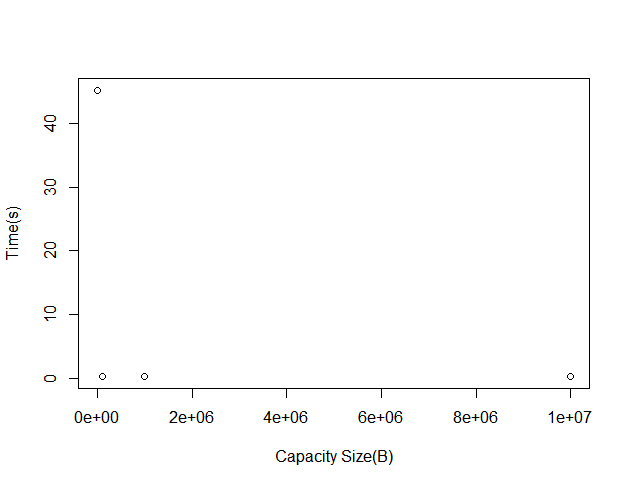
\includegraphics[width=8cm, height=6cm]{Time_Plot_Normal}
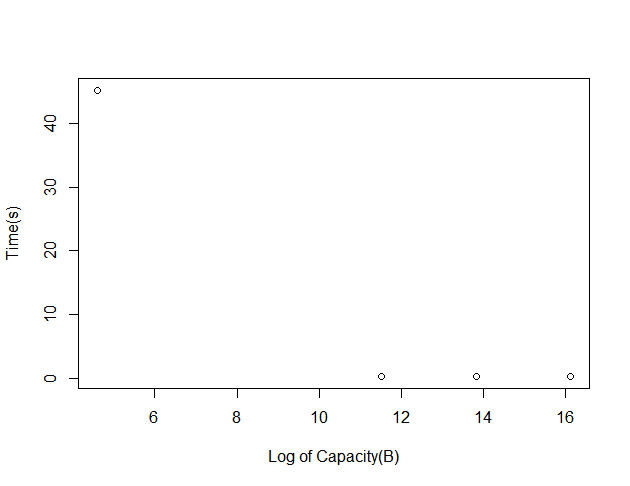
\includegraphics[width=8cm, height=6cm]{Time_Plot_xlog}
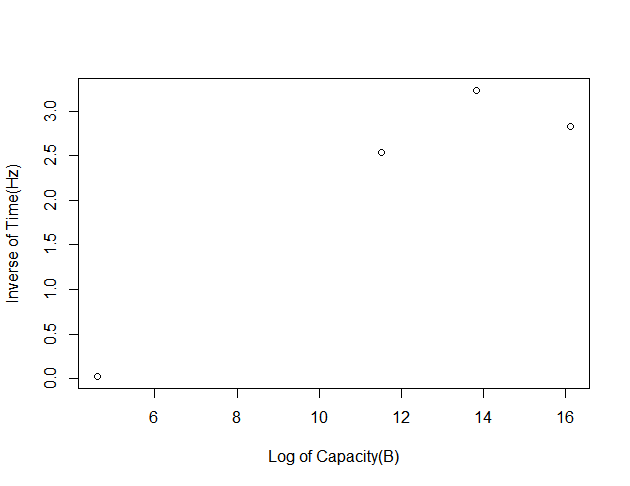
\includegraphics[width=8cm, height=6cm]{Time_Plot_xlog_y}
\end{center}

The link for the demo is here: https://youtu.be/eC4xV2\_kmtI

\end{document}